\documentclass{article}
\usepackage{amssymb,amsfonts,amsmath,amscd,amsthm}
\usepackage{graphicx}
\usepackage{parskip}
\usepackage{color}
\usepackage{bm}
\usepackage{booktabs}
\usepackage{fancyvrb}
\usepackage{booktabs}  %nice tables

\usepackage{tikz}
\usetikzlibrary{positioning}
\usepackage{verbatim}

\tikzset{
  % Specifications for style of nodes:
  base/.style = {
    rectangle,
    rounded corners,
    draw=black,
    text centered
  },
  chain/.style = {
    base,
    minimum width=5.5cm,
    minimum height=2cm,
    node distance=1cm,
    fill=orange!15
  },
  process/.style = {
    base,
    minimum width=1.5cm,
    minimum height=0.75cm,
    node distance=0.25cm,
    fill=blue!15
  },
  vector/.style = {
    rectangle,
    draw=black,
    minimum width=0.42cm,
    minimum height=0.42cm,
    node distance=0.0cm
  },
}

\def\parameter#1{
  \begin{scope}
    \node[vector, fill=green!40, right=of #1.west, xshift=0.11cm] (piece0) {};
    \node[vector, fill=yellow!40, right=of piece0.east, node distance=0cm] (piece1) {};
    \node[vector, fill=red!40, right=of piece1.east, node distance=0cm] (piece2) {};
  \end{scope}
}

\definecolor{dkgreen}{rgb}{0,0.6,0}
\definecolor{gray}{rgb}{0.5,0.5,0.5}
\definecolor{mauve}{rgb}{0.58,0,0.82}

\newcommand{\Quesoweb}{\url{https://github.com/libqueso}}
\newcommand{\Queso}{\texttt{QUESO}}
\newcommand{\QUESOversion}{0.51.0}

\usepackage{listings}          % to include codes using \lstinputlisting
\lstset{
language=c++,                  % choose the language of the code
basicstyle=\ttfamily,          % the size of the fonts that are used for the code
%stringstyle=\ttfamily,
%keywordstyle=\bfseries,       % so funciona com basicstyle=\footnotesize,\ttfamily se eu adicionar \usepackage{bold-extra}
keywordstyle=\color{blue},     % keyword style
commentstyle=\color{dkgreen},  % comment style
stringstyle=\color{mauve},
identifierstyle=\bfseries,
numberbychapter= true,
numberfirstline=false,
% numbers=left,                % where to put the line-numbers
numberstyle=\footnotesize,     % the size of the fonts that are used for the line-numbers
stepnumber=5,                  % the step between two line-numbers. If it is 1 each line will be numbered
numbersep=8pt,                 % how far the line-numbers are from the code
showspaces=false,              % show spaces adding particular underscores
showstringspaces=false,        % underline spaces within strings
showtabs=false,                % show tabs within strings adding particular underscores
tabsize=2,                     % sets default tabsize to 2 spaces
captionpos=b,                  % sets the caption-position to bottom
breaklines=true,               % sets automatic line breaking
breakatwhitespace=false,       % sets if automatic breaks should only happen at whitespace
escapeinside={\%*}{*)},        % if you want to add a comment within your code
morekeywords ={rm,ls},
belowskip = 10pt,              % \medskipamount%\smallskipamount,
aboveskip =10pt,
}

\title{Distributed parameter states in \Queso}
\author{Damon McDougall}

\begin{document}

\maketitle

\section{Introduction}

This document describes the current, serial, state of the parameter vector in
\Queso\ and makes a plan to transition to a distributed state.

\subsection{The current state}

The current state of the parameter vector in \Queso\ is serial.  Parallelism in
\Queso\ presents itself in two ways: 1) independent parallel Markov chains that
execute concurrently; and 2) a mechanism, an MPI communicator, that \Queso\
creates as part of the construction of \lstinline|FullEnvironment| the user can
hand to a forward problem demanding parallelism.  Neither of these parallel
capabilities distribute the parameter vector across multiple processes.  In
other words, each chain's process holds exactly the same parameter vector
value in the likelihood.

Here is some example commented code that executes the current situation:
\begin{lstlisting}
#include <queso/Environment.h>
#include <queso/GslVector.h>
#include <queso/GslMatrix.h>
#include <queso/ScalarFunction.h>
#include <queso/VectorSpace.h>
#include <queso/BoxSubset.h>

using namespace QUESO;

template <class V = GslVector, class M = GslMatrix>
class Likelihood : public BaseScalarFunction<V, M>
{
public:
  Likelihood(const char * prefix,
             const VectorSet<V, M> & domainSet)
    : BaseScalarFunction<V, M>(prefix, domainSet),
      m_env(domainSet.env())
  {
  }

  virtual double lnValue(const V & param) const
  {
    if (m_env.subRank() == 0) {
      std::cout << "Rank 0 param: " << param << '\n';
    }
    else {  // Rank 1
      std::cout << "Rank 1 param: " << param << '\n';
    }

    return 1.0;
  }

  virtual double actualValue(const V&, const V*, V*,
                             M*, V*) const
  {
    return 1.0;
  }

  const BaseEnvironment & m_env;
};

int main(int argc, char ** argv)
{
  // We'll assume the program was executed with
  // mpirun -np 2 and there's only one chain.

  MPI_Init(&argc, &argv);
  FullEnvironment env(MPI_COMM_WORLD, argv[1], "",
                      NULL);
  VectorSpace<> paramSpace(env, "", 2, NULL);
  GslVector min(paramSpace.zeroVector());
  GslVector max(paramSpace.zeroVector());
  min[0] = 0.0;
  min[1] = 0.0;
  max[0] = 1.0;
  max[1] = 1.0;
  BoxSubset<> paramDomain("", paramSpace, min, max);
  Likelihood<> likelihood("", paramDomain);

  GslVector point(paramSpace.zeroVector());
  point[0] = 0.5;
  point[1] = 0.5;
  likelihood.lnValue(point);  // Both ranks print the
                              // same parameter value

  MPI_Finalize();
  return 0;
}
\end{lstlisting}

\subsection{Why we need a distributed state}

There are some issues with a serial parameter vector, and some benefits to
moving to a distributed parameter vector.
\begin{itemize}
  \item There are problems with large parameter vectors (discretized fields)
    that necessitate distribution across multiple processes;
  \item Parallel parameter vector means \Queso\ can leverage existing high
    performance linear algebra packages for better compute resource usage;
  \item High performance linear algebra packages provide better performing
    optimization algorithms we could use before sampling;
  \item The serial implementation requires GSL, and GSL is licensed under the
    GPL.  We have customers at the labs that would like to ship \Queso\ as a
    binary and GPL third-party libraries prevent this from happening.
    \begin{itemize}
      \item A rebuttal to this point might be to use an alternative serial
        implementation with a more liberal license.  This is a reasonable
        suggestion but it doesn't address the first three points.
    \end{itemize}
\end{itemize}

\section{How the future might look}
\subsection{Parameter distribution in parallel}

If the user requests multiple processes per chain, then an approach we might
take is to distribute the parameter across those processes.  In the code
example above, that would mean process 0 sees only the first element of
\lstinline|point| and process 1 sees only the second element.  Here's a
depiction before the change:
%
\begin{center}
  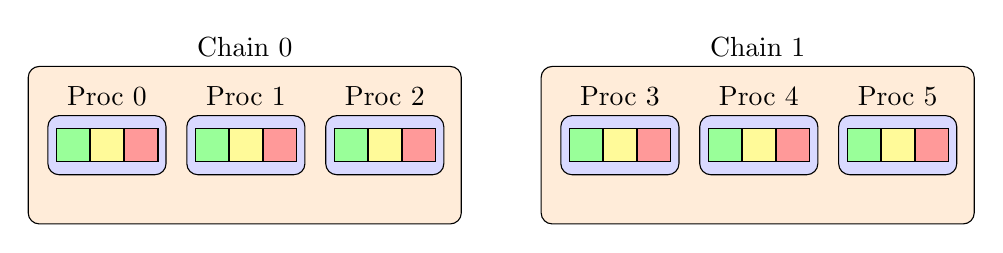
\begin{tikzpicture}
    % Specification of nodes (position, etc.)
    \node[chain, label={Chain 0}] (chain0) at (0, 0)                  {};
    \node[chain, label={Chain 1}, right=of chain0]         (chain1)   {};
    \node[process, label={Proc 0}, right=of chain0.west]   (process0) {};
    \node[process, label={Proc 1}, right=of process0.east] (process1) {};
    \node[process, label={Proc 2}, right=of process1.east] (process2) {};
    \node[process, label={Proc 3}, right=of chain1.west]   (process3) {};
    \node[process, label={Proc 4}, right=of process3.east] (process4) {};
    \node[process, label={Proc 5}, right=of process4.east] (process5) {};
    \parameter{process0}
    \parameter{process1}
    \parameter{process2}
    \parameter{process3}
    \parameter{process4}
    \parameter{process5}
  \end{tikzpicture}
\end{center}
%
And here's what it looks like after the change:
%
\begin{center}
  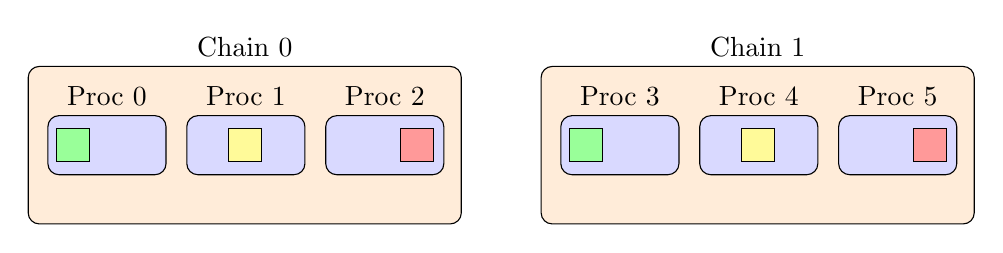
\begin{tikzpicture}
    % Specification of nodes (position, etc.)
    \node[chain, label={Chain 0}] (chain0) at (0, 0)                     {};
    \node[chain, label={Chain 1}, right=of chain0]         (chain1)      {};
    \node[process, label={Proc 0}, right=of chain0.west]   (process0)    {};
    \node[process, label={Proc 1}, right=of process0.east] (process1)    {};
    \node[process, label={Proc 2}, right=of process1.east] (process2)    {};
    \node[process, label={Proc 3}, right=of chain1.west]   (process3)    {};
    \node[process, label={Proc 4}, right=of process3.east] (process4)    {};
    \node[process, label={Proc 5}, right=of process4.east] (process5)    {};
    \node[vector, fill=green!40, right=of process0.west, xshift=0.11cm]  {};
    \node[vector, fill=yellow!40, right=of process1.west, xshift=0.53cm] {};
    \node[vector, fill=red!40, right=of process2.west, xshift=0.95cm]    {};
    \node[vector, fill=green!40, right=of process3.west, xshift=0.11cm]  {};
    \node[vector, fill=yellow!40, right=of process4.west, xshift=0.53cm] {};
    \node[vector, fill=red!40, right=of process5.west, xshift=0.95cm]    {};
  \end{tikzpicture}
\end{center}
%
Inside the likelihood the user is responsible for providing the mechanism
needed to pass the parameter information over to their forward model.  This
will not change in the case the parameter vector is distributed.  Therefore,
this is not a forwards-compatible change; parallel forward codes that worked
with a serial parameter vector and aren't designed to work with distributed
parameter vectors will fail or, worse, produce incorrect results.

What about the case where the user needs multiple independent model evaluations
for a single likelihood calculation?  This case arises when there are multiple
experimental data points.  It is reasonable to leverage independent concurrency
for these data points.  The diagram below depcits how the prcoesses may be
paritioned in this case.  The rows of processes in a chain correspond to those
needed by a single model evaluation.
%
\begin{center}
  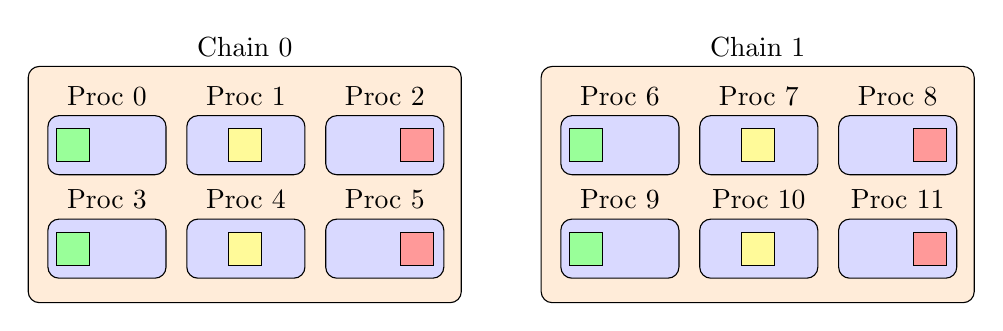
\begin{tikzpicture}
    % Specification of nodes (position, etc.)
    \node[chain, label={Chain 0}, minimum height=3cm]                      (chain0)    {};
    \node[process, label={Proc 0}, right=of chain0.west, yshift=0.5cm]     (process0)  {};
    \node[vector, fill=green!40, right=of process0.west, xshift=0.11cm]                {};
    \node[process, label={Proc 1}, right=of process0.east]                 (process1)  {};
    \node[vector, fill=yellow!40, right=of process1.west, xshift=0.53cm]               {};
    \node[process, label={Proc 2}, right=of process1.east]                 (process2)  {};
    \node[vector, fill=red!40, right=of process2.west, xshift=0.95cm]                  {};
    \node[process, label={Proc 3}, below=of process0.south, yshift=-0.3cm] (process3)  {};
    \node[vector, fill=green!40, right=of process3.west, xshift=0.11cm]                {};
    \node[process, label={Proc 4}, right=of process3.east]                 (process4)  {};
    \node[vector, fill=yellow!40, right=of process4.west, xshift=0.53cm]               {};
    \node[process, label={Proc 5}, right=of process4.east]                 (process5)  {};
    \node[vector, fill=red!40, right=of process5.west, xshift=0.95cm]                  {};
    \node[chain, label={Chain 1}, right=of chain0, minimum height=3cm]     (chain1)    {};
    \node[process, label={Proc 6}, right=of chain1.west, yshift=0.5cm]     (process6)  {};
    \node[vector, fill=green!40, right=of process6.west, xshift=0.11cm]                {};
    \node[process, label={Proc 7}, right=of process6.east]                 (process7)  {};
    \node[vector, fill=yellow!40, right=of process7.west, xshift=0.53cm]               {};
    \node[process, label={Proc 8}, right=of process7.east]                 (process8)  {};
    \node[vector, fill=red!40, right=of process8.west, xshift=0.95cm]                  {};
    \node[process, label={Proc 9}, below=of process6.south, yshift=-0.3cm] (process9)  {};
    \node[vector, fill=green!40, right=of process9.west, xshift=0.11cm]                {};
    \node[process, label={Proc 10}, right=of process9.east]                (process10) {};
    \node[vector, fill=yellow!40, right=of process10.west, xshift=0.53cm]              {};
    \node[process, label={Proc 11}, right=of process10.east]               (process11) {};
    \node[vector, fill=red!40, right=of process11.west, xshift=0.95cm]                 {};
  \end{tikzpicture}
\end{center}
%
Here the parameter vector is distributed over three processes; three process
are needed for a single model evaluation; and two model evaluations are needed
for a single likelihood evaluation.

The communicators \Queso\ ought to provide are: 1) for each chain all processes
belonging to that chain; 2) for each model evaluation needed for a likelihood
calculation, all processes needed for that model evaluation.  In the above
picture, \Queso\ will create six communicators; two chain communicators (one
for each chain) and four model communicators (for the two models evaluated
in each chain).

\subsection{Choice of parameter partitioning}

We noted in the previous subsection that the parameter vector is distributed
across the processes involved in a model evaluation.  This implies that if
there are multiplie independent model evaluations in a likelihood calculation
then we are not using these extra processes to house a piece of the parameter
vector.

For example, as depicted in the image above, the parameter is distributed
across three processes and not six.  Three processes are leveraged for a model
evaluation and two model evaluations per likelihood calculation.  This wasn't
the only choice we could have made.  We could have instead chosen to partition
the parameter vector across \emph{all} processes belonging to the chain.  The
above picture would look slightly different; the parameter vector would be
distributed across all six processes belonging to the chain communicator.

Once a model evaluation needs to be done, it is reasonable to expect that the
model communicator needs the entire (possibly distributed) parameter vector.
If the parameter vector is distributed across the entire chain communicator,
the user would be burdened with the point-to-point communication required to
organise the parameter vector for the model communicator.  The exact
point-to-point communication required depends on \emph{how} the parameter
vector is distributed and it may be done to minimise the user burden.

It ought to be clear at this point why we chose to distribute the parameter
vector among the model communicator and not the chain communicator.
Furthermore, it is reasonable to expect that, if the model already demands a
parallel environment, distributing the parameter over only the model
communicator is a reasonable choice.

\subsection{From the user's perspective}

There are a few things to look at:
\begin{enumerate}
  \item The parameter space
  \item The parameter domain
  \item Distributions on the domain (priors)
  \item Interacting with vectors and matrices
  \item The likelihood
\end{enumerate}
These should change as little as possible.

\subsubsection{The parameter space}

At present, the user calls the following to instantiate a parameter space of
dimension 2,
\begin{lstlisting}
MPI_Init(&argc, &argv);
FullEnvironment env(MPI_COMM_WORLD, argv[1], "",
                    NULL);
VectorSpace<> paramSpace(env, "", 2, NULL);
\end{lstlisting}
The parameter space is the same for each chain.  It is only \emph{within} a
chain that the parameter is paritioned.  There is a clear constraint here; the
number of processes belonging to the chain must divide the dimension of the
parameter space.  This might be problematic in the situation where the forward
model needs 10 processes to run quickly for a likelihood evaluation but the
user can't ask for more than 2 processes.

Can we avoid this constraint?  Maybe we allow the user to ask for more
processes per chain and just use a subset of them.  For example, if the user
asks for 10 processes per chain for the forward model evaluation then \Queso\
would also ask for how many of those the parameter should be distributed over.

\subsubsection{The parameter domain}

For a \lstinline|BoxSubset|, which is the most common domain, the user calls
\begin{lstlisting}
BoxSubset<> paramDomain("", paramSpace, min, max);
\end{lstlisting}
The parameter space is already partitioned and \lstinline|min| and
\lstinline|max| belong to the parameter space.  Everything is already set up
for the parameter domain and nothing needs to be done here from the user's
perspective.

What about other domains?  Another common domain is the
\lstinline|ConcatenatedSubset|.  What about user-defined domains?

\subsubsection{Distributions on partitioned domains}

As an example, a user might construct a Gaussian distribution for the prior.
The user calls
\begin{lstlisting}
GaussianVectorRV<> prior("", paramDomain, mean,
                         covariance);
\end{lstlisting}
From the user's perspective, nothing would need to change.  The mean belongs
to the already-partitioned parameter vector space, and so does the covariance
matrix.

Any distributions that rely on vectors or matrices for construction will lie
in the already-partitioned space and the user will see no changes in their
statistical application.

\subsubsection{Interacting with vectors and matrices}

It ought to be clear at this point that iteractions with distributed vectors
requires some care.  Since vector are distributed over processes belonging to
the chain, the following code
\begin{lstlisting}
GslVector<> v(paramSpace.zeroVector());
v[0] = 1.0;
\end{lstlisting}
will set local index 0 on process 0 and local index 0 on prcoessor 1.  Local
index 0 on processor 1 should map to global index 1 for \lstinline|v|.

Interacting with matrices has a similar story, but the paritioning for matrices
will happen over the rows.  The following code
\begin{lstlisting}
GslMatrix<> A(paramSpace.zeroVector());
A(0,0) = 1.0;
A(0,1) = 1.0;
\end{lstlisting}
will set local row index 0 on process 0 and local row index 0 on process 1.
Local row index 0 on process 1 maps to global row index 1 for \lstinline|A|.

\subsection{From \Queso's perspective}

\end{document}
